\mfpicnumber{1}
\opengraphsfile{RationalGraphs}

\setcounter{footnote}{0}

\label{RationalGraphs}

In this section, we take a closer look at graphing rational functions.  In Section \ref{IntroRational}, we learned that the graphs of rational functions may have holes in them and could have vertical, horizontal and slant asymptotes.  Theorems \ref{vavshole}, \ref{hathm} and \ref{sathm} tell us exactly when and where these behaviors will occur, and if we combine these results with what we already know about graphing functions, we will quickly be able to generate reasonable graphs of rational functions.  

\smallskip

One of the standard tools we will use is the sign diagram which was first introduced in Section \ref{Inequalities}, and then revisited in Section \ref{GraphsofPolynomials}.  In those sections, we operated under the belief that a function couldn't change its sign without its graph crossing through the $x$-axis.  The major theorem we used to justify this belief was the Intermediate Value Theorem, Theorem \ref{IVT}.   It turns out the Intermediate Value Theorem applies to all \textit{continuous} functions,\footnote{Recall that, for our purposes, this means the graphs are devoid of any breaks, jumps or holes} not just polynomials. Although rational functions are continuous on their domains,\footnote{Another result from Calculus.} Theorem \ref{vavshole} tells us that vertical asymptotes and holes occur at the values excluded from their domains.  In other words, rational functions aren't continuous at these excluded values which leaves open the possibility that the function could change sign \textit{without} crossing through the $x$-axis.  Consider the graph of $y=h(x)$ from Example \ref{ratfuncex}, recorded below for convenience.  We have added its $x$-intercept at $\left(\frac{1}{2},0\right)$ for the discussion that follows. Suppose we wish to construct a sign diagram for $h(x)$.    Recall that the intervals where $h(x)>0$, or $(+)$, correspond to the $x$-values where the graph of $y=h(x)$ is \textit{above} the $x$-axis; the intervals on which $h(x) < 0$, or $(-)$ correspond to where the graph is \textit{below} the $x$-axis.  

\smallskip

\begin{tabular}{m{1in}m{2.5in}m{2in}}

&

\begin{mfpic}[15]{-5}{5}{-7}{9}
\arrow \reverse \arrow \function{-5,-1.5,0.1}{(2*x-1)/(x+1)}
\arrow \reverse \arrow  \function{-0.63,5,0.1}{(2*x-1)/(x+1)}
\gclear \circle{(1,0.5),0.1}
\circle{(1,0.5),0.1}
\point[3pt]{(0.5,0)}
\dashed \polyline{(-5,2), (5,2)}
\dashed \polyline{(-1,-6), (-1,8)}
\tlabel[cc](5,-0.5){\scriptsize $x$}
\tlabel[cc](0.5,9){\scriptsize $y$}
\tlabel[cc](0.5,-0.6){\scriptsize $\frac{1}{2}$}
\axes
\xmarks{-4 step 1 until 4}
\ymarks{-6 step 1 until 8}
\tiny
\tlpointsep{4pt}
\axislabels {x}{ {$-4 \hspace{7pt}$} -4, {$-3\hspace{7pt}$} -3, {$-2\hspace{7pt}$} -2,  {$1$} 1, {$2$} 2, {$3$} 3, {$4$} 4}
\axislabels {y}{ {$\hspace{1in} -1$} -1, {$-2$} -2, {$-3$} -3, {$-4$} -4, {$-5$} -5, {$-6$} -6,  {$1$} 1, {$3$} 3, {$4$} 4, {$5$} 5, {$6$} 6, {$7$} 7, {$8$} 8}
\normalsize
\end{mfpic}

&

\begin{mfpic}[10]{-6.5}{6.5}{-2}{2}
\arrow \reverse \arrow \polyline{(-6.5,0),(6.5,0)}
\xmarks{-3,0,3}
\tlpointsep{6pt}
\axislabels {x}{{$-1$} -3, {$\frac{1}{2}$} 0, {$1$} 3 }
\tlabel[cc](-5,1){$(+)$}
\tlabel[cc](-3,1){\textinterrobang}
\tlabel[cc](-1.5,1){$(-)$}
\tlabel[cc](0,1){$0$}
\tlabel[cc](1.5,1){$(+)$}
\tlabel[cc](3,1){\textinterrobang}
\tlabel[cc](5,1){$(+)$}
\end{mfpic} 

\end{tabular}

\enlargethispage{.25in}
\vspace{-.1in}

As we examine the graph of $y=h(x)$, reading from left to right, we note that from $(-\infty,-1)$, the graph is above the $x$-axis, so $h(x)$ is $(+)$ there.  At $x=-1$, we have a vertical asymptote, at which point the graph `jumps' across the $x$-axis.  On the interval $\left(-1,\frac{1}{2}\right)$, the graph is below the $x$-axis, so $h(x)$ is $(-)$ there.  The graph crosses through the $x$-axis at $\left(\frac{1}{2},0\right)$ and remains above the $x$-axis until $x=1$, where we have a `hole' in the graph.  Since $h(1)$ is undefined, there is no sign here.  So we have $h(x)$ as $(+)$ on the interval $\left(\frac{1}{2}, 1\right)$.  Continuing, we see that on $(1, \infty)$, the graph of $y=h(x)$ is above the $x$-axis, so we mark $(+)$ there.  To construct a sign diagram from this information, we not only need to denote the zero of $h$, but also the places not in the domain of $h$.  As is our custom, we write `$0$' above $\frac{1}{2}$ on the sign diagram to remind us that it is a zero of $h$.  We need a different notation for $-1$ and $1$, and we have chosen to use `\textinterrobang' - a nonstandard symbol called the \href{http://en.wikipedia.org/wiki/Interrobang}{\underline{interrobang}}.  \index{interrobang} We use this symbol to convey a sense of surprise, caution and wonderment - an appropriate attitude to take when approaching these points.   The moral of the story is that when constructing sign diagrams for rational functions, we include the zeros as well as the values excluded from the domain.

\medskip

\phantomsection
\label{rationalsigndiagram}

\colorbox{ResultColor}{\bbm

\centerline{\textbf{Steps for Constructing a Sign Diagram for a  Rational Function}} 

\medskip

\hspace{.17in} Suppose $r$ is a rational function. \index{sign diagram ! rational function}

\begin{enumerate}

\item  Place any values excluded from the domain of  $r$ on the number line with an `\textinterrobang' above them.

\item  Find the zeros of $r$ and place them on the number line with the number $0$ above them.

\item  Choose a test value in each of the intervals determined in steps 1 and 2.

\item  Determine the sign of $r(x)$ for each test value in step 3, and write that sign above the corresponding interval.

\end{enumerate}

\ebm}

\medskip 

We now present our procedure for graphing rational functions and apply it to a few exhaustive examples.  Please note that we decrease the amount of detail given in the explanations as we move through the examples.  The reader should be able to fill in any details in those steps which we have abbreviated.

\medskip

\colorbox{ResultColor}{\bbm

\centerline{\textbf{Steps for Graphing Rational Functions}}

\medskip

\hspace{.17in} Suppose $r$ is a rational function. \index{graph ! rational function}

\begin{enumerate}

\item  Find the domain of $r$.

\item  Reduce $r(x)$ to lowest terms, if applicable.

\item  Find the $x$- and $y$-intercepts of the graph of $y=r(x)$, if they exist.

\item  Determine the location of any vertical asymptotes or holes in the graph, if they exist.  Analyze the behavior of $r$ on either side of the vertical asymptotes, if applicable.

\item  Analyze the end behavior of $r$.  Find the horizontal or slant asymptote, if one exists.

\item  Use a sign diagram and plot additional points, as needed, to sketch the graph of $y=r(x)$.

\end{enumerate}

\ebm}

\bigskip

\begin{ex}  Sketch a detailed graph of $f(x) = \dfrac{3x}{x^2-4}$.

\smallskip

{\bf Solution.}  We follow the six step procedure outlined above.

\begin{enumerate}

\item  As usual, we set the denominator equal to zero to get $x^2 - 4 = 0$.  We find $x = \pm 2$, so our domain is $(-\infty, -2) \cup (-2,2) \cup (2,\infty)$.

\item  To reduce $f(x)$ to lowest terms, we factor the numerator and denominator which yields $f(x) = \frac{3x}{(x-2)(x+2)}$.  There are no common factors which means $f(x)$ is already in lowest terms.

\item  To find the $x$-intercepts of the graph of $y=f(x)$, we set $y=f(x) = 0$.  Solving $ \frac{3x}{(x-2)(x+2)} = 0$ results in $x=0$.  Since $x=0$ is in our domain, $(0,0)$ is the $x$-intercept.  To find the $y$-intercept, we set $x=0$ and find $y = f(0) = 0$, so that $(0,0)$ is our $y$-intercept as well.\footnote{As we mentioned at least once earlier, since functions can have at most one $y$-intercept, once we find that $(0,0)$ is on the graph, we know it is the $y$-intercept.}

\item  The two numbers excluded from the domain of $f$ are $x = -2$ and $x=2$.  Since $f(x)$ didn't reduce at all, both of these values of $x$ still cause trouble in the denominator. Thus by Theorem \ref{vavshole}, $x=-2$ and $x=2$ are vertical asymptotes of the graph.  We can actually go a step further at this point and determine exactly how the graph approaches the asymptote near each of these values. Though not absolutely necessary,\footnote{The sign diagram in step 6 will also determine the behavior near the vertical asymptotes.} it is good practice for those heading off to Calculus.  For the discussion that follows, it is best to use the factored form of $f(x) = \frac{3x}{(x-2)(x+2)}$.

\begin{itemize}

\item  \textit{The behavior of $y=f(x)$ as $x \rightarrow -2$:}  Suppose $x \rightarrow -2^{-}$.  If we were to build a table of values, we'd use $x$-values a little less than $-2$, say $-2.1$, $-2.01$ and $-2.001$.  While there is no harm in actually building a table like we did in Section \ref{IntroRational}, we want to develop a `number sense' here.  Let's think about each factor in the formula of $f(x)$ as we imagine substituting a number like $x=-2.000001$ into $f(x)$. The quantity $3x$ would be very close to $-6$, the quantity $(x-2)$ would be very close to $-4$, and the factor $(x+2)$ would be very close to $0$.  More specifically, $(x+2)$ would be a little less than $0$, in this case, $-0.000001.$  We will call such a number a `very small $(-)$', `very small' meaning close to zero in absolute value. So, mentally, as $x \rightarrow -2^{-}$, we estimate  \[ f(x)   = \dfrac{3x}{(x-2)(x+2)} \approx \dfrac{-6}{(-4)\left( \mbox{very small $(-)$}\right)} = \dfrac{3}{2 \left( \mbox{very small $(-)$}\right)} \]  Now, the closer $x$ gets to $-2$, the smaller $(x+2)$ will become, so even though we are multiplying our `very small $(-)$' by $2$, the denominator will continue to get smaller and smaller, and remain negative.  The result is a fraction whose numerator is positive, but whose denominator is very small and negative.  Mentally, \[f(x) \approx \dfrac{3}{2 \left( \mbox{very small $(-)$}\right)} \approx \dfrac{3}{\mbox{very small $(-)$}} \approx \mbox{very big $(-)$}\]  The term `very big $(-)$' means a number with a large absolute value which is negative.\footnote{The actual retail value of $f(-2.000001)$ is approximately $-1,\!500,\!000$.}  What all of this means is that as $x \rightarrow -2^{-}$, $f(x) \rightarrow -\infty$.  Now suppose we wanted to determine the behavior of $f(x)$ as $x \rightarrow -2^{+}$.  If we imagine substituting something a little larger than $-2$ in for $x$, say $-1.999999$, we mentally estimate \[ f(x) \approx \dfrac{-6}{(-4)\left( \mbox{very small $(+)$}\right)} = \dfrac{3}{2 \left( \mbox{very small $(+)$}\right)}  \approx \dfrac{3}{\mbox{very small $(+)$}} \approx \mbox{very big $(+)$}\]  We conclude that as $x \rightarrow -2^{+}$, $f(x) \rightarrow \infty$.

\item  \textit{The behavior of $y=f(x)$ as $x \rightarrow 2$:} Consider $x \rightarrow 2^{-}$. We imagine substituting $x = 1.999999$.  Approximating $f(x)$ as we did above, we get \[ f(x) \approx \dfrac{6}{\left( \mbox{very small $(-)$}\right)(4)} = \dfrac{3}{2 \left( \mbox{very small $(-)$}\right)}  \approx \dfrac{3}{\mbox{very small $(-)$}} \approx \mbox{very big $(-)$}\]  We conclude that as $x \rightarrow 2^{-}$, $f(x) \rightarrow -\infty$.  Similarly, as $x \rightarrow 2^{+}$, we imagine substituting $x = 2.000001$ to get $f(x) \approx \frac{3}{\mbox{\scriptsize very small $(+)$}} \approx \mbox{very big (+)}$.  So as $x \rightarrow 2^{+}, f(x) \rightarrow \infty$.
\end{itemize}

Graphically, we have that near $x=-2$ and $x=2$ the graph of $y=f(x)$ looks like\footnote{We have deliberately left off the labels on the $y$-axis because we know only the behavior near $x=\pm 2$, not the actual function values.}

\begin{center}

\begin{mfpic}[15]{-4}{4}{-5}{5}
\arrow \curve{(-2.75,-3),(-2.5,-3.25), (-2.25,-4)}
\arrow \reverse \curve{(-1.75,4),(-1.5,3.25), (-1.25,3)}
\arrow \curve{(1.25,-3), (1.5,-3.25) , (1.75,-4)}
\arrow \curve{(2.75,3),(2.5,3.25), (2.25,4)}
\dashed \polyline{(-2,-4.5), (-2,4.5)}
\dashed \polyline{(2,-4.5), (2,4.5)}
\tlabel[cc](4,-0.5){\scriptsize $x$}
\tlabel[cc](0.5,5){\scriptsize $y$}
\axes
\xmarks{-3 step 1 until 3}
\tiny
\tlpointsep{4pt}
\axislabels {x}{ {$-3\hspace{7pt}$} -3, {$-1\hspace{7pt}$} -1,  {$1$} 1, {$3$} 3}
\normalsize
\end{mfpic}

\end{center}

\item  Next, we determine the end behavior of the graph of $y=f(x)$.  Since the degree of the numerator is $1$, and the degree of the denominator is $2$, Theorem \ref{hathm} tells us that $y=0$ is the horizontal asymptote.  As with the vertical asymptotes, we can glean more detailed information using `number sense'. For the discussion below, we use the formula $f(x) = \frac{3x}{x^2-4}$. 

\begin{itemize}

\item  \textit{The behavior of $y=f(x)$ as $x \rightarrow -\infty$:}  If we were to make a table of values to discuss the behavior of $f$ as $x \rightarrow -\infty$, we would substitute very `large' negative numbers in for $x$, say for example, $x = \mbox{$-1$ billion}$.  The numerator $3x$ would then be $-3 \, \mbox{billion}$, whereas the denominator $x^2-4$ would be $(\mbox{$-1$ billion})^2 - 4$, which is pretty much the same as  $1(\mbox{billion})^2$.  Hence, \[f\left(\mbox{$-1$ billion}\right) \approx \dfrac{-3 \, \mbox{billion}}{1(\mbox{billion})^2} \approx - \dfrac{3}{\mbox{billion}} \approx \mbox{very small $(-)$} \]

Notice that if we substituted in $x = \mbox{$-1$ trillion}$, essentially the same kind of cancellation would happen, and we would be left with an even `smaller' negative number.  This not only confirms the fact that as $x \rightarrow -\infty$, $f(x) \rightarrow 0$, it tells us that $f(x) \rightarrow 0^{-}$. In other words, the graph of $y=f(x)$ is a little bit \textit{below} the $x$-axis as we move to the far left.


\item  \textit{The behavior of $y=f(x)$ as $x \rightarrow \infty$:}  On the flip side, we can imagine substituting very large positive numbers in for $x$ and looking at the behavior of $f(x)$.   For example, let $x = \mbox{$1$ billion}$. Proceeding as before, we get \[f\left(\mbox{$1$ billion}\right) \approx \dfrac{3 \, \mbox{billion}}{1(\mbox{billion})^2} \approx \dfrac{3}{\mbox{billion}} \approx \mbox{very small $(+)$} \]  The larger the number we put in, the smaller the positive number we would get out.  In other words, as $x \rightarrow \infty$, $f(x) \rightarrow 0^{+}$, so the graph of $y=f(x)$ is a little bit \emph{above} the $x$-axis as we look toward the far right.

\end{itemize}

Graphically, we have\footnote{As with the vertical asymptotes in the previous step, we know only the behavior of the graph as $x \rightarrow \pm \infty$.  For that reason, we provide no $x$-axis labels.}

\begin{center}

\begin{mfpic}[15]{-4.75}{4.75}{-2}{2}
\arrow \curve{(2.5,0.85), (3,0.35), (4.25, 0.15)}
\arrow \curve{(-2.5,-0.85), (-3,-0.35), (-4.25, -0.15)}
\tlabel[cc](4.75,-0.5){\scriptsize $x$}
\tlabel[cc](0.5,2){\scriptsize $y$}
\axes
\ymarks{-1 step 1 until 1}
\tiny
\tlpointsep{4pt}
\axislabels {y}{{$-1$} -1, {$1$} 1}
\normalsize
\end{mfpic}

\end{center}

\item  Lastly, we construct a sign diagram for $f(x)$.  The $x$-values excluded from the domain of $f$ are $x = \pm 2$, and the only zero of $f$ is $x=0$.  Displaying these appropriately on the number line gives us four test intervals, and we choose the test values\footnote{In this particular case, we can eschew test values, since our analysis of the behavior of $f$ near the vertical asymptotes and our end behavior analysis have given us the signs on each of the test intervals.  In general, however, this won't always be the case, so for demonstration purposes, we continue with our usual construction.} $x=-3$, $x=-1$, $x=1$ and $x=3$.  We find $f(-3)$ is $(-)$, $f(-1)$ is $(+)$, $f(1)$ is $(-)$ and $f(3)$ is $(+)$.  Combining this with our previous work, we get the graph of $y=f(x)$ below. 

\begin{tabular}{m{0.5in}m{2in}m{2.5in}}

&

\begin{mfpic}[10]{-6}{6}{-2}{2}
\arrow \reverse \arrow \polyline{(-6,0),(6,0)}
\xmarks{-3,0,3}
\arrow \polyline{(-4.5,-1.5),(-4.5,-0.5)}
\arrow \polyline{(-1.5,-1.5),(-1.5,-0.5)}
\arrow \polyline{(1.5,-1.5),(1.5,-0.5)}
\arrow \polyline{(4.5,-1.5),(4.5,-0.5)}
\tlpointsep{4pt}
\axislabels {x}{{$-2$} -3, {$0$} 0, {$2$} 3 }
\tlabel[cc](-4.5,1){$(-)$}
\tlabel[cc](-4.5,-2.25){$-3$}
\tlabel[cc](-3,1){\textinterrobang}
\tlabel[cc](-1.5,1){$(+)$}
\tlabel[cc](-1.75,-2.25){$-1$}
\tlabel[cc](0,1){$0$}
\tlabel[cc](1.5,1){$(-)$}
\tlabel[cc](1.5,-2.25){$1$}
\tlabel[cc](3,1){\textinterrobang}
\tlabel[cc](4.5,1){$(+)$}
\tlabel[cc](4.5,-2.25){$3$}
\end{mfpic} 

&

\begin{mfpic}[16]{-6}{6}{-4}{4}
\arrow \reverse \arrow \function{-6, -2.5, 0.1}{(3*x)/((x**2)-4)}
\arrow \reverse \arrow \function{-1.5, 1.5, 0.1}{(3*x)/((x**2)-4)}
\arrow \reverse \arrow \function{2.5, 6, 0.1}{(3*x)/((x**2)-4)}
\point[3pt]{(0,0)}
\dashed \polyline{(-2,-4), (-2,4)}
\dashed \polyline{(2,-4), (2,4)}
\tlabel[cc](6,-0.5){\scriptsize $x$}
\tlabel[cc](0.5,4){\scriptsize $y$}
\axes
\xmarks{-5 step 1 until 5}
\ymarks{-3 step 1 until 3}
\tiny
\tlpointsep{4pt}
 \axislabels {x}{ {$-5\hspace{7pt}$} -5, {$-4 \hspace{7pt}$} -4 ,{$-3\hspace{7pt}$} -3, {$-1\hspace{7pt}$} -1,  {$1$} 1, {$3$} 3,  {$4$} 4, {$5$} 5}
\axislabels {y}{ {$-3$} -3, {$-2$} -2,{$-1$} -1, {$1$} 1, {$2$} 2,{$3$} 3}
\normalsize
\end{mfpic}

\end{tabular}

\end{enumerate}

\qed

\end{ex}

A couple of notes are in order.  First, the graph of $y=f(x)$ certainly seems to possess symmetry with respect to the origin.  In fact, we can check $f(-x) = -f(x)$ to see that $f$ is an odd function.  In some textbooks, checking for symmetry is part of the standard procedure for graphing rational functions; but since it happens comparatively rarely\footnote{And Jeff doesn't think much of it to begin with...} we'll just point it out when we see it.  Also note that while $y=0$ is the horizontal asymptote, the graph of $f$ actually crosses the $x$-axis at $(0,0)$.  The myth that graphs of rational functions can't cross their horizontal asymptotes is completely false,\footnote{That's why we called it a MYTH!} as we shall see again in our next example.

\begin{ex}  Sketch a detailed graph of $g(x) = \dfrac{2x^2-3x-5}{x^2-x-6}$.

{\bf Solution.}

\begin{enumerate}

\item  Setting $x^2-x-6 = 0$ gives $x = -2$ and $x=3$.  Our domain is $(-\infty, -2) \cup (-2,3) \cup (3,\infty)$.

\item  Factoring $g(x)$ gives $g(x) = \frac{(2x-5)(x+1)}{(x-3)(x+2)}$.  There is no cancellation, so $g(x)$ is in lowest terms.

\item  To find the $x$-intercept  we set $y = g(x) = 0$.  Using the factored form of $g(x)$ above, we find the zeros to be the solutions of $(2x-5)(x+1)=0$.  We obtain $x = \frac{5}{2}$ and $x=-1$. Since both of these numbers are in the domain of $g$, we have two $x$-intercepts, $\left( \frac{5}{2},0\right)$ and $(-1,0)$.  To find the $y$-intercept, we set $x=0$ and find $y = g(0) = \frac{5}{6}$, so our $y$-intercept is $\left(0, \frac{5}{6}\right)$.

\item  Since $g(x)$ was given to us in lowest terms, we have, once again by Theorem \ref{vavshole} vertical asymptotes $x=-2$ and $x=3$.  Keeping in mind $g(x) = \frac{(2x-5)(x+1)}{(x-3)(x+2)}$, we proceed to our analysis near each of these values.

\begin{itemize}

\item  \textit{The behavior of $y=g(x)$ as $x \rightarrow -2$:}  As $x \rightarrow -2^{-}$, we imagine substituting a number a little bit less than $-2$. We have \[g(x) \approx \frac{(-9)(-1)}{(-5)(\mbox{very small $(-)$})} \approx \frac{9}{\mbox{very small $(+)$}} \approx \mbox{very big (+)}\] so as $x \rightarrow -2^{-}$, $g(x) \rightarrow \infty$. On the flip side, as $x \rightarrow -2^{+}$, we get \[g(x) \approx \frac{9}{\mbox{ very small $(-)$}} \approx \mbox{very big $(-)$}\] so $g(x) \rightarrow -\infty$.

\item  \textit{The behavior of $y=g(x)$ as $x \rightarrow 3$:}  As $x \rightarrow 3^{-}$, we imagine plugging in a number just shy  of $3$. We have \[g(x) \approx \frac{(1)(4)}{(\mbox{ very small $(-)$}) (5)} \approx \frac{4}{\mbox{very small $(-)$}} \approx \mbox{very big $(-)$}\] Hence, as $x \rightarrow 3^{-}$, $g(x) \rightarrow -\infty$. As $x \rightarrow 3^{+}$, we get \[g(x) \approx \frac{4}{\mbox{ very small $(+)$}} \approx \mbox{very big $(+)$}\] so $g(x) \rightarrow \infty$.

\end{itemize}

Graphically, we have (again, without labels on the $y$-axis)


\begin{center}

\begin{mfpic}[15]{-5}{5}{-5}{5}
\arrow \curve{(-2.75,3),(-2.5,3.25), (-2.25,4)}
\arrow \reverse \curve{(-1.75,-4),(-1.5,-3.25), (-1.25,-3)}
\arrow \curve{(2.25,-3), (2.5,-3.25) , (2.75,-4)}
\arrow \curve{(3.75,3),(3.5,3.25), (3.25,4)}
\dashed \polyline{(-2,-4.5), (-2,4.5)}
\dashed \polyline{(3,-4.5), (3,4.5)}
\tlabel[cc](5,-0.5){\scriptsize $x$}
\tlabel[cc](0.5,5){\scriptsize $y$}
\axes
\xmarks{-4 step 1 until 4}
\tiny
\tlpointsep{4pt}
\axislabels {x}{ {$-3\hspace{7pt}$} -3, {$-1\hspace{7pt}$} -1,  {$1$} 1, {$2$} 2, {$4$} 4}
\normalsize
\end{mfpic}

\end{center}


\item  Since the degrees of the numerator and denominator of $g(x)$ are the same, we know from Theorem \ref{hathm} that we can find the horizontal asymptote of the graph of $g$ by taking the ratio of the leading terms coefficients, $y = \frac{2}{1} = 2$.  However, if we take the time to do a more detailed analysis, we will be able to reveal some `hidden' behavior which would be lost otherwise.\footnote{That is, if you use a calculator to graph. Once again, Calculus is the ultimate graphing power tool.}  As in the discussion following Theorem \ref{hathm}, we use the result of the long division $\left(2x^2-3x-5\right) \div \left(x^2-x-6\right)$ to rewrite $g(x) = \frac{2x^2-3x-5}{x^2-x-6}$ as $g(x) = 2 - \frac{x-7}{x^2-x-6}.$  We focus our attention on the term $\frac{x-7}{x^2-x-6}$.  

\begin{itemize}

\item  \textit{The behavior of $y=g(x)$ as $x \rightarrow -\infty$:} If imagine substituting $x = \mbox{$-1$ billion}$ into $\frac{x-7}{x^2-x-6}$, we estimate $\frac{x-7}{x^2-x-6} \approx \frac{\mbox{\scriptsize $-1$ billion}}{1 \mbox{\scriptsize billion}^2} \approx \mbox{very small $(-)$}$.\footnote{In the denominator, we would have $(1 \mbox{billion})^2 - 1 \mbox{billion} - 6$. It's easy to see why the $6$ is insignificant, but to ignore the $1$ billion seems criminal.  However, compared to ($1$ billion)$^{2}$, it's on the insignificant side;  it's $10^{18}$ versus $10^9$.  We are once again using the fact that for polynomials, end behavior is determined by the leading term, so in the denominator, the $x^2$ term wins out over the $x$ term.}  Hence, \[g(x) =  2 - \frac{x-7}{x^2-x-6} \approx 2 - \mbox{very small $(-)$} = 2 + \mbox{very small $(+)$}\]  In other words, as $x \rightarrow -\infty$, the graph of $y=g(x)$ is a little bit \textit{above} the line $y=2$.

\item  \textit{The behavior of $y=g(x)$ as $x \rightarrow \infty$.}  To consider $\frac{x-7}{x^2-x-6}$ as $x \rightarrow \infty$, we imagine substituting $x = \mbox{$1$ billion}$ and, going through the usual mental routine, find \[\frac{x-7}{x^2-x-6} \approx \mbox{very small $(+)$}\]  Hence, $g(x) \approx 2 - \ \mbox{very small $(+)$}$, in other words, the graph of $y=g(x)$ is just \textit{below} the line $y=2$ as $x \rightarrow \infty$.

\end{itemize}

On $y=g(x)$, we have (again, without labels on the $x$-axis)


\begin{center}

\begin{mfpic}[15]{-4.75}{4.75}{-1}{3}
\arrow \curve{(2.5,1.15), (3,1.65), (4.25, 1.85)}
\arrow \curve{(-2.5,2.85), (-3,2.35), (-4.25, 2.15)}
\dashed \polyline{(-4.75,2), (4.75,2)}
\tlabel[cc](4.75,-0.5){\scriptsize $x$}
\tlabel[cc](0.5,3){\scriptsize $y$}
\axes
\ymarks{-1 step 1 until 1}
\tiny
\tlpointsep{4pt}
\axislabels {y}{{$-1$} -1, {$1$} 1}
\normalsize
\end{mfpic}

\end{center}

\item  Finally we construct our sign diagram.  We place an `\textinterrobang' above $x=-2$ and $x=3$, and a `$0$' above $x = \frac{5}{2}$ and $x=-1$.  Choosing test values in the test intervals gives us $f(x)$ is $(+)$ on the intervals $(-\infty, -2)$, $\left(-1, \frac{5}{2}\right)$ and $(3, \infty)$, and $(-)$ on the intervals $(-2,-1)$ and $\left(\frac{5}{2}, 3\right)$.  As we piece together all of the information, we note that the graph must cross the horizontal asymptote at some point after $x=3$ in order for it to approach $y=2$ from underneath.  This is the subtlety that we would have missed had we skipped the long division and subsequent end behavior analysis.  We can, in fact, find exactly when the graph crosses $y=2$.  As a result of the long division, we have $g(x) =  2 - \frac{x-7}{x^2-x-6}$.  For $g(x) = 2$, we would need $\frac{x-7}{x^2-x-6} = 0$. This gives $x-7= 0$, or $x=7$.  Note that $x-7$ is the remainder when $2x^2-3x-5$ is divided by $x^2-x-6$, so it makes sense that for $g(x)$ to equal the quotient $2$, the remainder from the division must be $0$.  Sure enough, we find $g(7)=2$.  Moreover, it stands to reason that $g$ must attain a relative minimum at some point past $x=7$.  Calculus verifies that at $x=13$, we have such a minimum at exactly $(13, 1.96)$.  The reader is challenged to find calculator windows which show the graph crossing its horizontal asymptote on one window, and the relative minimum in the other.

\begin{tabular}{m{0.05in}m{2.5in}m{2.5in}}

&

\begin{mfpic}[10]{-8}{7}{-2}{2}
\arrow \reverse \arrow \polyline{(-8,0),(7,0)}
\xmarks{-5,-2,1,4}
\tlpointsep{4pt}
\axislabels {x}{{$-2$} -5, {$-1$} -2, {$\frac{5}{2}$} 1, {$3$} 4}
\tlabel[cc](-6.5,1){$(+)$}
\tlabel[cc](-5,1){\textinterrobang}
\tlabel[cc](-3.5,1){$(-)$}
\tlabel[cc](-2,1){$0$}
\tlabel[cc](-0.5,1){$(+)$}
\tlabel[cc](1,1){$0$}
\tlabel[cc](2.5,1){$(-)$}
\tlabel[cc](4,1){\textinterrobang}
\tlabel[cc](5.5,1){$(+)$}
\end{mfpic}

& 

\begin{mfpic}[10]{-10}{10}{-5}{9}
\arrow \reverse \arrow \function{-9, -2.29, 0.1}{(2*(x**2)-3*x-5)/((x**2)-x-6)}
\arrow \reverse \arrow \function{-1.69, 2.86, 0.1}{(2*(x**2)-3*x-5)/((x**2)-x-6)}
\arrow \reverse \arrow \function{3.12, 9, 0.1}{(2*(x**2)-3*x-5)/((x**2)-x-6)}
\point[3pt]{(-1,0), (2.5,0), (0, 0.83333)}
\dashed \polyline{(-2,-5), (-2,9)}
\dashed \polyline{(3,-5), (3,9)}
\dashed \polyline{(-10,2), (10,2)}
\tlabel[cc](10,-0.5){\scriptsize $x$}
\tlabel[cc](0.5,9){\scriptsize $y$}
\axes
\xmarks{-9 step 1 until 9}
\ymarks{-4 step 1 until 8}
\tiny
\tlpointsep{4pt}
\axislabels {x}{ {$-9\hspace{7pt}$} -9, {$-8 \hspace{7pt}$} -8 ,{$-7 \hspace{7pt}$} -7, {$-6 \hspace{7pt}$} -6,{$-5\hspace{7pt}$} -5, {$-4 \hspace{7pt}$} -4 ,{$-3\hspace{7pt}$} -3, {$-1\hspace{7pt}$} -1,  {$1$} 1, {$2$} 2,  {$4$} 4, {$5$} 5, {$6$} 6,  {$7$} 7, {$8$} 8, {$9$} 9}
\axislabels {y}{ {$-4$} -4,{$-3$} -3, {$-2$} -2,{$-1$} -1, {$1$} 1, {$3$} 3, {$4$} 4, {$5$} 5, {$6$} 6, {$7$} 7, {$8$} 8}
\normalsize
\end{mfpic}

\end{tabular}

\end{enumerate}

\qed

\end{ex}


Our next example gives us an opportunity to more thoroughly analyze a slant asymptote.

\begin{ex}  Sketch a detailed graph of $h(x) = \dfrac{2x^3+5x^2+4x+1}{x^2+3x+2}$.

{ \bf Solution.}  

\begin{enumerate}

\item  For domain, you know the drill.  Solving $x^2+3x+2 = 0$ gives $x = -2$ and $x=-1$.  Our answer is $(-\infty, -2) \cup (-2, -1) \cup (-1, \infty)$.

\item  To reduce $h(x)$, we need to factor the numerator and denominator.  To factor the numerator, we use the techniques\footnote{Bet you never thought you'd never see \textit{that} stuff again before the Final Exam!} set forth in Section \ref{RealZeros} and we get  \[h(x) =  \dfrac{2x^3+5x^2+4x+1}{x^2+3x+2} = \dfrac{(2x+1)(x+1)^2}{(x+2)(x+1)} = \dfrac{ (2x+1) (x+1)^{\cancelto{1}{2}}  }{(x+2)\cancel{(x+1)}} = \dfrac{(2x+1)(x+1)}{x+2} \]

We will use this reduced formula for $h(x)$ as long as we're not substituting $x=-1$.  To make this exclusion specific, we write $h(x) = \frac{(2x+1)(x+1)}{x+2}$, $x \neq -1$.

\item  To find the $x$-intercepts, as usual, we set $h(x) = 0$ and solve.  Solving $\frac{(2x+1)(x+1)}{x+2}=0$ yields $x=-\frac{1}{2}$ and $x=-1$.  The latter isn't in the domain of $h$, so we exclude it.  Our only $x$-intercept is $\left(-\frac{1}{2}, 0\right)$.  To find the $y$-intercept, we set $x=0$.  Since $0 \neq -1$, we can use the reduced formula for $h(x)$ and we get $h(0) = \frac{1}{2}$ for a $y$-intercept of $\left(0,\frac{1}{2}\right)$.

\item  From Theorem \ref{vavshole}, we know that since $x=-2$ still poses a threat in the denominator of the reduced function, we have a vertical asymptote there.  As for $x=-1$, the factor $(x+1)$ was canceled from the denominator when we reduced $h(x)$, so it no longer causes trouble there.  This means that we get a hole when $x=-1$.  To find the $y$-coordinate of the hole, we substitute $x=-1$ into $\frac{(2x+1)(x+1)}{x+2}$, per Theorem \ref{vavshole} and get $0$.  Hence, we have a hole on the $x$-axis at $(-1,0)$.  It should make you uncomfortable plugging $x=-1$ into the reduced formula for $h(x)$, especially since we've made such a big deal concerning the stipulation about not letting $x=-1$ for that formula.  What we are really doing is taking a Calculus short-cut to the more detailed kind of analysis near $x=-1$ which we will show below.  Speaking of which, for the discussion that follows,  we will use the formula $h(x) = \frac{(2x+1)(x+1)}{x+2}$, $x \neq -1$.

\begin{itemize}

\item  \textit{The behavior of $y=h(x)$ as $x \rightarrow -2$:}  As $x \rightarrow -2^{-}$, we imagine substituting a number a little bit less than $-2$. We have $h(x) \approx \frac{(-3)(-1)}{(\mbox{\scriptsize very small $(-)$})} \approx \frac{3}{(\mbox{\scriptsize very small $(-)$})}\approx \mbox{very big $(-)$}$ thus as $x \rightarrow -2^{-}$, $h(x) \rightarrow -\infty$. On the other side of $-2$, as $x \rightarrow -2^{+}$, we find that $h(x) \approx \frac{3}{\mbox{\scriptsize very small $(+)$}} \approx \mbox{very big $(+)$}$, so $h(x) \rightarrow \infty$.

\item  \textit{The behavior of $y=h(x)$ as $x \rightarrow -1$.}  As $x \rightarrow -1^{-}$, we imagine plugging in a number a bit less than $x=-1$. We have $h(x) \approx \frac{(-1)(\mbox{\scriptsize very small $(-)$})}{1} = \mbox{very small $(+)$}$ Hence, as $x \rightarrow -1^{-}$, $h(x) \rightarrow 0^{+}$. This means that as $x \rightarrow -1^{-}$, the graph is a bit above the point $(-1,0)$.  As $x \rightarrow -1^{+}$, we get $h(x) \approx \frac{(-1)(\mbox{\scriptsize very small $(+)$})}{1} = \mbox{very small $(-)$}$.  This gives us that as $x \rightarrow -1^{+}$, $h(x) \rightarrow 0^{-}$, so the graph is a little bit lower than $(-1,0)$ here.  

\end{itemize}

Graphically, we have

\begin{center}

\begin{mfpic}[15]{-4}{1}{-5}{5}
\arrow \curve{(-2.75,-3),(-2.5,-3.25), (-2.25,-4)}
\arrow \reverse \curve{(-1.75,4),(-1.5,3.25), (-1.25,3)}
\curve{(-1.25,0.5), (-1,0), (-0.75,-0.5)}
\dashed \polyline{(-2,-4.5), (-2,4.5)}
\tlabel[cc](1,-0.5){\scriptsize $x$}
\tlabel[cc](0.5,5){\scriptsize $y$}
\axes
\xmarks{-2,-1}
\tiny
\tlpointsep{4pt}
\axislabels {x}{ {$-3\hspace{7pt}$} -3}
\normalsize
\gclear \circle{(-1,0),0.1}
\circle{(-1,0),0.1}
\end{mfpic}

\end{center}

\item  For end behavior, we note that the degree of the numerator of $h(x)$, $2x^3+5x^2+4x+1$, is $3$ and the degree of the denominator, $x^2+3x+2$, is $2$ so by Theorem \ref{sathm}, the graph of $y = h(x)$ has a slant asymptote.  For $x\rightarrow \pm \infty$, we are far enough away from $x=-1$ to use the reduced formula, $h(x) = \frac{(2x+1)(x+1)}{x+2}$, $x \neq -1$.  To perform long division, we multiply out the numerator and get $h(x) = \frac{2x^2+3x+1}{x+2}$, $x \neq -1$, and rewrite $h(x) = 2x-1+\frac{3}{x+2}$, $x \neq -1$.  By Theorem \ref{sathm}, the slant asymptote is $y = 2x-1$, and to better see \textit{how} the graph approaches the asymptote, we focus our attention on the term generated from the remainder, $\frac{3}{x+2}$.

\begin{itemize}

\item  \textit{The behavior of $y=h(x)$ as $x \rightarrow -\infty$:} Substituting  $x = \mbox{$-1$ billion}$ into $\frac{3}{x+2}$, we get the estimate $\frac{3}{\mbox{\scriptsize $-1$ billion}} \approx \mbox{very small $(-)$}$.  Hence, $h(x) = 2x-1+\frac{3}{x+2} \approx 2x-1 + \mbox{very small $(-)$}$.  This means the graph of $y=h(x)$ is a little bit \textit{below} the line $y=2x-1$ as $x \rightarrow -\infty$.

\item  \textit{The behavior of $y=h(x)$ as $x \rightarrow \infty$:}  If $x \rightarrow \infty$, then $\frac{3}{x+2} \approx \mbox{very small $(+)$}$.  This means $h(x) \approx 2x-1 + \mbox{very small $(+)$}$, or that the graph of $y=h(x)$ is a little bit \textit{above} the line $y=2x-1$ as $x \rightarrow \infty$.

\end{itemize}

 Graphically we have

\begin{center}

\begin{mfpic}[15]{-4.75}{4.75}{-4.75}{4.75}
\arrow \curve{(-1.25,-4), (-1.5,-4.2), (-1.7, -4.75)}
\arrow \curve{(2.25,4), (2.5,4.2), (2.75, 4.75)}
\dashed \function{-1.7,2.7,0.1}{2*x-1}
\tlabel[cc](4.75,-0.5){\scriptsize $x$}
\tlabel[cc](0.5,4.75){\scriptsize $y$}
\axes
\ymarks{-4 step 4 until 1}
\tiny
\tlpointsep{4pt}
\axislabels {y}{{$-4$} -4,{$-3$} -3,{$-2$} -2,{$-1$} -1, {$1$} 1, {$2$} 2, {$3$} 3, {$4$} 4}
\normalsize
\end{mfpic}

\end{center}

\item  To make our sign diagram, we place an `\textinterrobang' above $x=-2$ and $x=-1$ and a `$0$' above $x=-\frac{1}{2}$.  On our four test intervals, we find $h(x)$ is $(+)$ on $(-2,-1)$ and $\left(-\frac{1}{2}, \infty\right)$ and $h(x)$ is $(-)$ on $(-\infty, -2)$ and $\left(-1,-\frac{1}{2}\right)$.  Putting all of our work together yields the graph below.

\end{enumerate}

\begin{tabular}{m{0.5in}m{2in}m{2.5in}}

&

\begin{mfpic}[10]{-8}{8}{-2}{2}
\arrow \reverse \arrow \polyline{(-8,0),(8,0)}
\xmarks{-4,0,4}
\tlpointsep{6pt}
\axislabels {x}{{$-2 \hspace{9pt}$} -4, {$-1 \hspace{9pt}$} 0, {$-\frac{1}{2} \hspace{9pt}$} 4}
\tlabel[cc](-6,1){$(-)$}
\tlabel[cc](-4,1){\textinterrobang}
\tlabel[cc](-2.25,1){$(+)$}
\tlabel[cc](0,1){\textinterrobang}
\tlabel[cc](2.25,1){$(-)$}
\tlabel[cc](4,1){$0$}
\tlabel[cc](6,1){$(+)$}
\end{mfpic} 

&

\begin{mfpic}[16][8]{-5}{5}{-15}{10}
\arrow \reverse \arrow \function{-6.67, -2.32, 0.1}{(2*(x**2)+3*x+1)/(x+2)}
\arrow \reverse \arrow \function{-1.79, 5.29, 0.1}{(2*(x**2)+3*x+1)/(x+2)}
\point[3pt]{(-0.5,0)}
\dashed \polyline{(-2,-15), (-2,10)}
\dashed \function{-7,5.5,0.1}{2*x-1}
\tlabel[cc](5,-0.5){\scriptsize $x$}
\tlabel[cc](0.5,10){\scriptsize $y$}
\axes
\xmarks{-4 step 1 until 4}
\ymarks{-14 step 1 until 9}
\tiny
\tlpointsep{4pt}
\axislabels {x}{{$-4 \hspace{7pt}$} -4 ,{$-3\hspace{7pt}$} -3, {$-1\hspace{7pt}$} -1,  {$1$} 1,{$2$} 2, {$3$} 3,  {$4$} 4}
\axislabels {y}{ {$-14$} -14, {$-13$} -13,{$-12$} -12,{$-11$} -11, {$-10$} -10,{$-9$} -9,{$-8$} -8, {$-7$} -7,{$-6$} -6,{$-5$} -5, {$-4$} -4,{$-3$} -3, {$-2$} -2,{$-1$} -1, {$1$} 1, {$2$} 2,{$3$} 3, {$4$} 4,{$5$} 5, {$6$} 6,{$7$} 7, {$8$} 8,{$9$} 9}
\normalsize
\gclear \ellipse{(-1,0),0.1,0.2}
\ellipse{(-1,0),0.1,0.2}
\end{mfpic}

\end{tabular}

We could ask whether the graph of $y=h(x)$ crosses its slant asymptote.  From the formula $h(x) = 2x-1+\frac{3}{x+2}$, $x \neq -1$, we see that if $h(x) = 2x-1$, we would have $\frac{3}{x+2} = 0$.  Since this will never happen, we conclude the graph never crosses its slant asymptote.\footnote{But rest assured, some graphs do!}
\qed


\end{ex}

We end this section with an example that shows it's not all pathological weirdness when it comes to rational functions and technology still has a role to play in studying their graphs at this level.

\begin{ex}  \label{calcisneededhere} Sketch the graph of $r(x) = \dfrac{x^4+1}{x^2+1}$.

\smallskip

{\bf Solution.}

\begin{enumerate}

\item  The denominator $x^2+1$ is never zero so the domain is $(-\infty, \infty)$.

\item  With no real zeros in the denominator, $x^2+1$ is an irreducible quadratic.  Our only hope of reducing $r(x)$ is if $x^2+1$ is a factor of $x^4+1$.  Performing long division gives us \[\frac{x^4+1}{x^2+1} = x^2-1+\frac{2}{x^2+1}\] The remainder is not zero so $r(x)$ is already reduced.

\item  To find the $x$-intercept, we'd set $r(x) = 0$.  Since there are no real solutions to $\frac{x^4+1}{x^2+1}=0$, we have no $x$-intercepts.  Since $r(0) = 1$, we get $(0,1)$ as the $y$-intercept.

\item  This step doesn't apply to $r$, since its domain is all real numbers.

\item  For end behavior, we note that since the degree of the numerator is exactly \textit{two} more than the degree of the denominator, neither Theorems \ref{hathm} nor \ref{sathm} apply.\footnote{This won't stop us from giving it the old community college try, however!} We know from our attempt to reduce $r(x)$ that we can rewrite $r(x) = x^2-1+\frac{2}{x^2+1}$, so we focus our attention on the term corresponding to the remainder, $\frac{2}{x^2+1}$  It should be clear that as $x \rightarrow \pm \infty$, $\frac{2}{x^2+1} \approx \mbox{very small $(+)$}$, which means $r(x) \approx x^2-1 + \mbox{very small $(+)$}$.  So the graph $y=r(x)$ is a little bit \textit{above} the graph of the parabola $y=x^2-1$ as $x \rightarrow \pm \infty$. Graphically,

\begin{center}

\begin{mfpic}[15]{-3}{3}{-2}{6}
\dashed \function{-2.5,2.5,0.1}{x**2-1}
\arrow \curve{(-2,4), (-2.25,4.5), (-2.5,6)}
\arrow \curve{(2,4), (2.25,4.5), (2.5,6)}
\axes
\ymarks{-1,1,2,3,4,5}
\tiny
\tlpointsep{4pt}
\axislabels {y}{ {$1$} 1, {$2$} 2,{$3$} 3, {$4$} 4,{$5$} 5}
\normalsize 
\tlabel[cc](3,-0.5){\scriptsize $x$}
\tlabel[cc](0.5,6){\scriptsize $y$}
\end{mfpic}

\end{center}

\item  There isn't much work to do for a sign diagram for $r(x)$, since its domain is all real numbers and it has no zeros.  Our sole test interval is $(-\infty, \infty)$, and since we know $r(0) = 1$, we conclude $r(x)$ is $(+)$ for all real numbers. At this point, we don't have much to go on for a graph.\footnote{So even Jeff at this point may check for symmetry!  We leave it to the reader to show $r(-x) = r(x)$ so $r$ is even, and, hence, its graph is symmetric about the $y$-axis.} Below is a comparison of what we have determined analytically versus what the calculator shows us.  We have no way to detect the relative extrema analytically\footnote{Without appealing to Calculus, of course.} apart from brute force plotting of points, which is done more efficiently by the calculator.

\end{enumerate}

\begin{tabular}{m{1in}m{2in}m{3in}}

&

\begin{mfpic}[15]{-4}{4}{-2}{7}
\arrow \reverse \arrow \function{-2.5, 2.5, 0.1}{0.75*(x**2)+1}
\dashed \function{-2.5, 2.5, 0.1}{x^2-1}
\point[3pt]{(0,1)}
\tlabel[cc](3,-0.5){\scriptsize $x$}
\tlabel[cc](0.5,6){\scriptsize $y$}
\axes
\xmarks{-3 step 1 until 3}
\ymarks{-1 step 1 until 5}
\tiny
\tlpointsep{4pt}
\axislabels {x}{{$-3\hspace{7pt}$} -3, {$-1\hspace{7pt}$} -1,  {$1$} 1,{$2$} 2, {$3$} 3}
\axislabels {y}{ {$1$} 1, {$2$} 2,{$3$} 3, {$4$} 4,{$5$} 5, {$6$} 6}
\normalsize
\end{mfpic} 

&

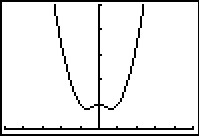
\includegraphics[width=2in]{./RationalsGraphics/Rationals09.jpg}

\end{tabular}

\end{ex}

\vspace{-.35in} \qed

\medskip

As usual, the authors offer no apologies for what may be construed as `pedantry' in this section.  We feel that the detail presented in this section is necessary to obtain a firm grasp of the concepts presented here and it also serves as an introduction to the methods employed in Calculus.  As we have said many times in the past, your instructor will decide how much, if any, of the kinds of details presented here are `mission critical' to your understanding of Precalculus. Without further delay, we present you with this section's Exercises.

\newpage

\subsection{Exercises}

In Exercises \ref{sixstepfirst} - \ref{sixsteplast}, use the six-step procedure to graph the rational function.  Be sure to draw any asymptotes as dashed lines.

\begin{multicols}{2}
\begin{enumerate}

\item $f(x) = \dfrac{4}{x + 2}$ \label{sixstepfirst}
\item $f(x) = \dfrac{5x}{6 - 2x}$

\setcounter{HW}{\value{enumi}}
\end{enumerate}
\end{multicols}

\begin{multicols}{2}
\begin{enumerate}
\setcounter{enumi}{\value{HW}}

\item $f(x) = \dfrac{1}{x^{2}}$
\item $f(x) = \dfrac{1}{x^{2} + x - 12}$

\setcounter{HW}{\value{enumi}}
\end{enumerate}
\end{multicols}

\begin{multicols}{2}
\begin{enumerate}
\setcounter{enumi}{\value{HW}}

\item $f(x) = \dfrac{2x - 1}{-2x^{2} - 5x + 3}$
\item $f(x) = \dfrac{x}{x^{2} + x - 12}$ \vphantom{$\dfrac{2x}{2x}$}

\setcounter{HW}{\value{enumi}}
\end{enumerate}
\end{multicols}

\begin{multicols}{2}
\begin{enumerate}
\setcounter{enumi}{\value{HW}}

\item $f(x) = \dfrac{4x}{x^2+4}$
\item $f(x) = \dfrac{4x}{x^2-4}$

\setcounter{HW}{\value{enumi}}
\end{enumerate}
\end{multicols}

\begin{multicols}{2}
\begin{enumerate}
\setcounter{enumi}{\value{HW}}

\item $f(x) = \dfrac{x^2-x-12}{x^2+x-6}$
\item $f(x) = \dfrac{3x^2-5x-2}{x^2-9}$

\setcounter{HW}{\value{enumi}}
\end{enumerate}
\end{multicols}

\begin{multicols}{2}
\begin{enumerate}
\setcounter{enumi}{\value{HW}}

\item $f(x) = \dfrac{x^2-x-6}{x+1}$

\item $f(x) = \dfrac{x^2-x}{3-x}$

\setcounter{HW}{\value{enumi}}
\end{enumerate}
\end{multicols}

\begin{multicols}{2}
\begin{enumerate}
\setcounter{enumi}{\value{HW}}

\item $f(x) = \dfrac{x^3+2x^2+x}{x^2-x-2}$

\item $f(x) = \dfrac{-x^{3} + 4x}{x^{2} - 9}$

\setcounter{HW}{\value{enumi}}
\end{enumerate}
\end{multicols}

\begin{multicols}{2}
\begin{enumerate}
\setcounter{enumi}{\value{HW}}

\item  $f(x) = \dfrac{x^3-2x^2+3x}{2x^2+2}$

\item \hspace{-0.1in}\footnote{Once you've done the six-step procedure, use your calculator to graph this function on the viewing window $[0, 12] \times [0, 0.25]$.  What do you see?} $f(x) = \dfrac{x^{2} - 2x + 1}{x^{3} + x^{2} - 2x}$ \label{sixsteplast}

\setcounter{HW}{\value{enumi}}
\end{enumerate}
\end{multicols}

In Exercises \ref{usetransratfirst} - \ref{usetransratlast}, graph the rational function by applying transformations to the graph of $y = \dfrac{1}{x}$.

\begin{multicols}{2}
\begin{enumerate}
\setcounter{enumi}{\value{HW}}

\item $f(x) = \dfrac{1}{x - 2}$ \label{usetransratfirst}
\item $g(x) = 1 - \dfrac{3}{x}$

\setcounter{HW}{\value{enumi}}
\end{enumerate}
\end{multicols}

\begin{multicols}{2}
\begin{enumerate}
\setcounter{enumi}{\value{HW}}


\item $h(x) = \dfrac{-2x + 1}{x}$ (Hint: Divide)
\item $j(x) = \dfrac{3x - 7}{x - 2}$ (Hint: Divide) \label{usetransratlast}


\setcounter{HW}{\value{enumi}}
\end{enumerate}
\end{multicols}


\begin{enumerate}
\setcounter{enumi}{\value{HW}}

\item Discuss with your classmates how you would graph $f(x) = \dfrac{ax + b}{cx + d}$.  What restrictions must be placed on $a, b, c$ and $d$ so that the graph is indeed a transformation of $y = \dfrac{1}{x}$?

\item In Example \ref{intropolyexample} in Section \ref{GraphsofPolynomials} we showed that $p(x) = \frac{4x+x^3}{x}$ is not a polynomial even though its formula reduced to $4 + x^{2}$ for $x \neq 0$.  However, it is a rational function similar to those studied in the section.  With the help of your classmates, graph $p(x)$.

\item Let $g(x) = \displaystyle \frac{x^{4} - 8x^{3} + 24x^{2} - 72x + 135}{x^{3} - 9x^{2} + 15x - 7}.\;$  With the help of your classmates, find the $x$- and $y$- intercepts of the graph of $g$.  Find the intervals on which the function is increasing, the intervals on which it is decreasing and the local extrema. Find all of the asymptotes of the graph of $g$ and any holes in the graph, if they exist.  Be sure to show all of your work including any polynomial or synthetic division.  Sketch the graph of $g$, using more than one picture if necessary to show all of the important features of the graph.

\setcounter{HW}{\value{enumi}}
\end{enumerate}

Example \ref{calcisneededhere} showed us that the six-step procedure cannot tell us everything of importance about the graph of a rational function.  Without Calculus, we need to use our graphing calculators to reveal the hidden mysteries of rational function behavior.  Working with your classmates, use a graphing calculator to examine the graphs of the rational functions given in Exercises \ref{rationalneedcalcfirst} - \ref{rationalneedcalclast}.  Compare and contrast their features.  Which features can the six-step process reveal and which features cannot be detected by it?

\begin{multicols}{4}
\begin{enumerate}
\setcounter{enumi}{\value{HW}}

\item $f(x) = \dfrac{1}{x^{2} + 1}$ \vphantom{$\dfrac{2x^{3}}{2x^{2}}$}  \label{rationalneedcalcfirst}
\item $f(x) = \dfrac{x}{x^{2} + 1}$ \vphantom{$\dfrac{2x^{3}}{2x^{2}}$}
\item $f(x) = \dfrac{x^{2}}{x^{2} + 1}$ \vphantom{$\dfrac{2x^{3}}{2x^{2}}$}
\item $f(x) = \dfrac{x^{3}}{x^{2} + 1}$ \vphantom{$\dfrac{2x^{3}}{2x^{2}}$} \label{rationalneedcalclast}

\setcounter{HW}{\value{enumi}}
\end{enumerate}
\end{multicols}

\newpage

\subsection{Answers}

\begin{enumerate}

\item \begin{multicols}{2} \raggedcolumns
$f(x) = \dfrac{4}{x + 2}$\\
Domain: $(-\infty, -2) \cup (-2, \infty)$\\
No $x$-intercepts\\
$y$-intercept: $(0, 2)$\\
Vertical asymptote: $x = -2$\\
As $x \rightarrow -2^{-}, \; f(x) \rightarrow -\infty$\\
As $x \rightarrow -2^{+}, \; f(x) \rightarrow \infty$\\
Horizontal asymptote: $y = 0$\\
As $x \rightarrow -\infty, \; f(x) \rightarrow 0^{-}$\\
As $x \rightarrow \infty, \; f(x) \rightarrow 0^{+}$\\

\begin{mfpic}[10]{-8}{6}{-6}{6}
\arrow \reverse \arrow \function{-8,-2.7,0.1}{4/(x+2)}
\arrow \reverse \arrow  \function{-1.3,6,0.1}{4/(x+2)}
\point[3pt]{(0,2)}
\dashed \polyline{(-2,-6), (-2,6)}
\tlabel[cc](6,-0.5){\scriptsize $x$}
\tlabel[cc](0.5,6){\scriptsize $y$}
\axes
\xmarks{-7 step 1 until 5}
\ymarks{-5 step 1 until 5}
\tiny
\tlpointsep{4pt}
\axislabels {x}{{$-7 \hspace{7pt}$} -7, {$-6 \hspace{7pt}$} -6, {$-5 \hspace{7pt}$} -5, {$-4 \hspace{7pt}$} -4, {$-3\hspace{7pt}$} -3, {$-2\hspace{7pt}$} -2, {$-1\hspace{7pt}$} -1,  {$1$} 1, {$2$} 2, {$3$} 3, {$4$} 4, {$5$} 5}
\axislabels {y}{{$-5$} -5, {$-4$} -4, {$-3$} -3, {$-2$} -2, {$-1$} -1, {$1$} 1, {$2$} 2, {$3$} 3, {$4$} 4, {$5$} 5}
\normalsize
\end{mfpic}

\end{multicols}

\item \begin{multicols}{2} \raggedcolumns 
$f(x) = \dfrac{5x}{6 - 2x}$\\
Domain: $(-\infty, 3) \cup (3, \infty)$\\
$x$-intercept: $(0, 0)$\\
$y$-intercept: $(0, 0)$\\
Vertical asymptote: $x = 3$\\
As $x \rightarrow 3^{-}, \; f(x) \rightarrow \infty$\\
As $x \rightarrow 3^{+}, \; f(x) \rightarrow -\infty$\\
Horizontal asymptote: $y = -\frac{5}{2}$\\
As $x \rightarrow -\infty, \; f(x) \rightarrow -\frac{5}{2}^{+}$\\
As $x \rightarrow \infty, \; f(x) \rightarrow -\frac{5}{2}^{-}$\\

\begin{mfpic}[10]{-4}{10}{-8}{4}
\arrow \reverse \arrow \function{-4,1.8,0.1}{(5*x)/(6 - (2*x))}
\arrow \reverse \arrow  \function{4.4,10,0.1}{(5*x)/(6 - (2*x))}
\point[3pt]{(0,0)}
\dashed \polyline{(3,-8), (3,4)}
\dashed \polyline{(-4,-2.5), (10,-2.5)}
\tlabel[cc](10,-0.5){\scriptsize $x$}
\tlabel[cc](0.5,4){\scriptsize $y$}
\axes
\xmarks{-3 step 1 until 9}
\ymarks{-7 step 1 until 3}
\tiny
\tlpointsep{4pt}
\axislabels {x}{{$-3\hspace{7pt}$} -3, {$-2\hspace{7pt}$} -2, {$-1\hspace{7pt}$} -1,  {$1$} 1, {$2$} 2, {$3$} 3, {$4$} 4, {$5$} 5, {$6$} 6, {$7$} 7, {$8$} 8, {$9$} 9}
\axislabels {y}{{$-7$} -7, {$-6$} -6, {$-5$} -5, {$-4$} -4, {$-3$} -3, {$-2$} -2, {$-1$} -1, {$1$} 1, {$2$} 2, {$3$} 3}
\normalsize
\end{mfpic}

\end{multicols}

\item \begin{multicols}{2} \raggedcolumns 
$f(x) = \dfrac{1}{x^{2}}$\\
Domain: $(-\infty, 0) \cup (0, \infty)$\\
No $x$-intercepts\\
No $y$-intercepts\\
Vertical asymptote: $x = 0$\\
As $x \rightarrow 0^{-}, \; f(x) \rightarrow \infty$\\
As $x \rightarrow 0^{+}, \; f(x) \rightarrow \infty$\\
Horizontal asymptote: $y = 0$\\
As $x \rightarrow -\infty, \; f(x) \rightarrow 0^{+}$\\
As $x \rightarrow \infty, \; f(x) \rightarrow 0^{+}$\\

\begin{mfpic}[15][20]{-5}{5}{-1}{6}
\arrow \reverse \arrow \function{-5,-0.42,0.1}{1/(x**2)}
\arrow \reverse \arrow  \function{0.42,5,0.1}{1/(x**2)}
\tlabel[cc](5,-0.5){\scriptsize $x$}
\tlabel[cc](0.5,6){\scriptsize $y$}
\axes
\xmarks{-4 step 1 until 4}
\ymarks{1 step 1 until 5}
\tiny
\tlpointsep{4pt}
\axislabels {x}{{$-4 \hspace{7pt}$} -4, {$-3\hspace{7pt}$} -3, {$-2\hspace{7pt}$} -2, {$-1\hspace{7pt}$} -1,  {$1$} 1, {$2$} 2, {$3$} 3, {$4$} 4}
\axislabels {y}{{$1$} 1, {$2$} 2, {$3$} 3, {$4$} 4, {$5$} 5}
\normalsize
\end{mfpic}

\end{multicols}

\pagebreak

\item \begin{multicols}{2} \raggedcolumns 
$f(x) = \dfrac{1}{x^{2} + x - 12} = \dfrac{1}{(x - 3)(x + 4)}$\\
Domain: $(-\infty, -4) \cup (-4, 3) \cup (3, \infty)$\\
No $x$-intercepts\\
$y$-intercept: $(0, -\frac{1}{12})$\\
Vertical asymptotes: $x = -4$ and $x = 3$\\
As $x \rightarrow -4^{-}, \; f(x) \rightarrow \infty$\\
As $x \rightarrow -4^{+}, \; f(x) \rightarrow -\infty$\\
As $x \rightarrow 3^{-}, \; f(x) \rightarrow -\infty$\\
As $x \rightarrow 3^{+}, \; f(x) \rightarrow \infty$\\
Horizontal asymptote: $y = 0$\\
As $x \rightarrow -\infty, \; f(x) \rightarrow 0^{+}$\\
As $x \rightarrow \infty, \; f(x) \rightarrow 0^{+}$\\

\begin{mfpic}[13][50]{-7}{5}{-1.5}{1.5}
\arrow \reverse \arrow \function{-6.5,-4.15,0.1}{1/((x**2) + x - 12)}
\arrow \reverse \arrow  \function{-3.85, 2.85,0.1}{1/((x**2) + x - 12)}
\arrow \reverse \arrow  \function{3.15,4.5,0.1}{1/((x**2) + x - 12)}
\point[3pt]{(0,-0.08333)}
\dashed \polyline{(3,-1.5), (3,1.5)}
\dashed \polyline{(-4,-1.5), (-4,1.5)}
\tlabel[cc](5,-0.1){\scriptsize $x$}
\tlabel[cc](0.5,1.5){\scriptsize $y$}
\axes
\xmarks{-6 step 1 until 4}
\ymarks{-1 step 1 until 1}
\tiny
\tlpointsep{4pt}
\axislabels {x}{{$-6 \hspace{7pt}$} -6, {$-5 \hspace{7pt}$} -5, {$-4 \hspace{7pt}$} -4, {$-3\hspace{7pt}$} -3, {$-2\hspace{7pt}$} -2, {$-1\hspace{7pt}$} -1,  {$1$} 1, {$2$} 2, {$3$} 3, {$4$} 4}
\axislabels {y}{{$-1$} -1, {$1$} 1}
\normalsize
\end{mfpic}

\end{multicols}

\item \begin{multicols}{2} \raggedcolumns 
$f(x) = \dfrac{2x - 1}{-2x^{2} - 5x + 3} = -\dfrac{2x - 1}{(2x - 1)(x + 3)}$\\
Domain: $(-\infty, -3) \cup (-3, \frac{1}{2}) \cup (\frac{1}{2}, \infty)$\\
No $x$-intercepts\\
$y$-intercept: $(0, -\frac{1}{3})$\\
$f(x) = \dfrac{-1}{x + 3}, \; x \neq \frac{1}{2}$\\
Hole in the graph at $(\frac{1}{2}, -\frac{2}{7})$\\
Vertical asymptote: $x = -3$\\
As $x \rightarrow -3^{-}, \; f(x) \rightarrow \infty$\\
As $x \rightarrow -3^{+}, \; f(x) \rightarrow -\infty$\\
Horizontal asymptote: $y = 0$\\
As $x \rightarrow -\infty, \; f(x) \rightarrow 0^{+}$\\
As $x \rightarrow \infty, \; f(x) \rightarrow 0^{-}$\\

\begin{mfpic}[15][45]{-8}{3}{-2}{2}
\arrow \reverse \arrow \function{-8,-3.5,0.1}{-1/(x+3)}
\arrow \reverse \arrow  \function{-2.5,3,0.1}{-1/(x+3)}
\dashed \polyline{(-3,-2), (-3,2)}
\gclear \ellipse{(0.5,-0.2857),0.1,0.033}
\ellipse{(0.5,-0.2857),0.1,0.033}
\point[3pt]{(0,-0.333)}
\tlabel[cc](3,0.1){\scriptsize $x$}
\tlabel[cc](0.5,2){\scriptsize $y$}
\axes
\xmarks{-7 step 1 until 2}
\ymarks{-1,1}
\tiny
\tlpointsep{4pt}
\axislabels {x}{{$-7 \hspace{7pt}$} -7, {$-6 \hspace{7pt}$} -6, {$-5 \hspace{7pt}$} -5, {$-4 \hspace{7pt}$} -4, {$-3\hspace{7pt}$} -3, {$-2\hspace{7pt}$} -2, {$-1\hspace{7pt}$} -1,  {$1$} 1, {$2$} 2}
\axislabels {y}{{$-1$} -1, {$1$} 1}
\normalsize
\end{mfpic}

\end{multicols}

\item \begin{multicols}{2} \raggedcolumns 
$f(x) = \dfrac{x}{x^{2} + x - 12} = \dfrac{x}{(x - 3)(x + 4)}$\\
Domain: $(-\infty, -4) \cup (-4, 3) \cup (3, \infty)$\\
$x$-intercept: $(0, 0)$\\
$y$-intercept: $(0, 0)$\\
Vertical asymptotes: $x = -4$ and $x = 3$\\
As $x \rightarrow -4^{-}, \; f(x) \rightarrow -\infty$\\
As $x \rightarrow -4^{+}, \; f(x) \rightarrow \infty$\\
As $x \rightarrow 3^{-}, \; f(x) \rightarrow -\infty$\\
As $x \rightarrow 3^{+}, \; f(x) \rightarrow \infty$\\
Horizontal asymptote: $y = 0$\\
As $x \rightarrow -\infty, \; f(x) \rightarrow 0^{-}$\\
As $x \rightarrow \infty, \; f(x) \rightarrow 0^{+}$\\

\begin{mfpic}[13][50]{-7}{6}{-1.5}{1.5}
\arrow \reverse \arrow \function{-6.5,-4.4,0.1}{x/((x**2) + x - 12)}
\arrow \reverse \arrow  \function{-3.6, 2.72,0.1}{x/((x**2) + x - 12)}
\arrow \reverse \arrow  \function{3.35,5.5,0.1}{x/((x**2) + x - 12)}
\point[3pt]{(0,0)}
\dashed \polyline{(3,-1.5), (3,1.5)}
\dashed \polyline{(-4,-1.5), (-4,1.5)}
\tlabel[cc](6,-0.1){\scriptsize $x$}
\tlabel[cc](0.5,1.5){\scriptsize $y$}
\axes
\xmarks{-6 step 1 until 5}
\ymarks{-1 step 1 until 1}
\tiny
\tlpointsep{4pt}
\axislabels {x}{{$-6 \hspace{7pt}$} -6, {$-5 \hspace{7pt}$} -5, {$-4 \hspace{7pt}$} -4, {$-3\hspace{7pt}$} -3, {$-2\hspace{7pt}$} -2, {$-1\hspace{7pt}$} -1,  {$1$} 1, {$2$} 2, {$3$} 3, {$4$} 4, {$5$} 5}
\axislabels {y}{{$-1$} -1, {$1$} 1}
\normalsize
\end{mfpic}

\end{multicols}

\item \begin{multicols}{2} \raggedcolumns
$f(x) = \dfrac{4x}{x^{2} + 4}$\\
Domain: $(-\infty,  \infty)$\\
$x$-intercept:  $(0,0)$\\
$y$-intercept:  $(0,0)$\\
No vertical asymptotes \\
No holes in the graph\\
Horizontal asymptote: $y = 0$ \\
As $x \rightarrow -\infty, f(x) \rightarrow 0^{-}$\\
As $x \rightarrow \infty, f(x) \rightarrow 0^{+}$\\

\begin{mfpic}[10][25]{-8}{8}{-2}{2}
\arrow \reverse \arrow \function{-8,8,0.1}{(4*x)/((x**2)+4)}
\point[3pt]{(0,0)}
\tlabel[cc](8,-0.5){\scriptsize $x$}
\tlabel[cc](0.5,2){\scriptsize $y$}
\axes
\xmarks{-7 step 1 until 7}
\ymarks{-1 step 1 until 1}
\tiny
\tlpointsep{4pt}
\axislabels {x}{{$-7 \hspace{7pt}$} -7,{$-6 \hspace{7pt}$} -6,{$-5 \hspace{7pt}$} -5, {$-4 \hspace{7pt}$} -4, {$-3\hspace{7pt}$} -3, {$-2\hspace{7pt}$} -2, {$-1\hspace{7pt}$} -1,  {$1$} 1, {$2$} 2, {$3$} 3, {$4$} 4, {$5$} 5, {$6$} 6, {$7$} 7}
\axislabels {y}{{$-1$} -1, {$1$} 1}
\normalsize
\end{mfpic}


\end{multicols}

\item \begin{multicols}{2} \raggedcolumns
$f(x) = \dfrac{4x}{x^{2} -4} = \dfrac{4x}{(x + 2)(x - 2)}$\\
Domain: $(-\infty, -2) \cup (-2, 2) \cup (2, \infty)$\\
$x$-intercept:  $(0,0)$\\
$y$-intercept:  $(0,0)$\\
Vertical asymptotes: $x = -2, x = 2$\\
As $x \rightarrow -2^{-}, f(x) \rightarrow -\infty$\\
As $x \rightarrow -2^{+}, f(x) \rightarrow \infty$\\
As $x \rightarrow 2^{-}, f(x) \rightarrow -\infty$\\
As $x \rightarrow 2^{+}, f(x) \rightarrow \infty$\\
No holes in the graph\\
Horizontal asymptote: $y = 0$ \\
As $x \rightarrow -\infty, f(x) \rightarrow 0^{-}$\\
As $x \rightarrow \infty, f(x) \rightarrow 0^{+}$\\

\begin{mfpic}[15]{-6}{6}{-6}{6}
\arrow \reverse \arrow \function{-6,-2.4,0.1}{(4*x)/((x**2)-4)}
\arrow \reverse \arrow \function{-1.64,1.64,0.1}{(4*x)/((x**2)-4)}
\arrow \reverse \arrow \function{-6,-2.4,0.1}{(4*x)/((x**2)-4)}
\arrow \reverse \arrow \function{2.4,6,0.1}{(4*x)/((x**2)-4)}
\point[3pt]{(0,0)}
\dashed \polyline{(-2,-6), (-2,6)}
\dashed \polyline{(2,-6), (2,6)}
\tlabel[cc](6,-0.5){\scriptsize $x$}
\tlabel[cc](0.5,6){\scriptsize $y$}
\axes
\xmarks{-5 step 1 until 5}
\ymarks{-5 step 1 until 5}
\tiny
\tlpointsep{4pt}
\axislabels {x}{{$-5 \hspace{7pt}$} -5, {$-4 \hspace{7pt}$} -4, {$-3\hspace{7pt}$} -3, {$-2\hspace{7pt}$} -2, {$-1\hspace{7pt}$} -1,  {$1$} 1, {$2$} 2, {$3$} 3, {$4$} 4, {$5$} 5}
\axislabels {y}{{$-5$} -5, {$-4$} -4, {$-3$} -3, {$-2$} -2, {$-1$} -1, {$1$} 1, {$2$} 2, {$3$} 3, {$4$} 4, {$5$} 5}
\normalsize
\end{mfpic}
\end{multicols}

\item \begin{multicols}{2} \raggedcolumns

$f(x) = \dfrac{x^2-x-12}{x^{2} +x - 6} = \dfrac{x-4}{x - 2} \, x \neq -3$\\
Domain: $(-\infty, -3) \cup (-3, 2) \cup (2, \infty)$\\
$x$-intercept:  $(4,0)$\\
$y$-intercept:  $(0,2)$\\
Vertical asymptote: $x = 2$\\
As $x \rightarrow 2^{-}, f(x) \rightarrow \infty$\\
As $x \rightarrow 2^{+}, f(x) \rightarrow -\infty$\\
Hole at $\left(-3, \frac{7}{5} \right)$ \\
Horizontal asymptote: $y = 1$ \\
As $x \rightarrow -\infty, f(x) \rightarrow 1^{+}$\\
As $x \rightarrow \infty, f(x) \rightarrow 1^{-}$\\


\begin{mfpic}[15]{-6}{6}{-6}{6}
\arrow \reverse \arrow \function{-6,1.5,0.1}{(x-4)/(x-2)}
\arrow \reverse \arrow \function{2.333,6,0.1}{(x-4)/(x-2)}
\point[3pt]{(4,0), (0,2)}
\gclear \circle{(-3,1.4),0.1}
\circle{(-3,1.4),0.1}
\dashed \polyline{(2,-6), (2,6)}
\dashed \polyline{(-6,1), (6,1)}
\tlabel[cc](6,-0.5){\scriptsize $x$}
\tlabel[cc](0.5,6){\scriptsize $y$}
\axes
\xmarks{-5 step 1 until 5}
\ymarks{-5 step 1 until 5}
\tiny
\tlpointsep{4pt}
\axislabels {x}{{$-5 \hspace{7pt}$} -5, {$-4 \hspace{7pt}$} -4, {$-3\hspace{7pt}$} -3, {$-2\hspace{7pt}$} -2, {$-1\hspace{7pt}$} -1,  {$1$} 1, {$2$} 2, {$3$} 3, {$4$} 4, {$5$} 5}
\axislabels {y}{{$-5$} -5, {$-4$} -4, {$-3$} -3, {$-2$} -2, {$-1$} -1, {$1$} 1, {$2$} 2, {$3$} 3, {$4$} 4, {$5$} 5}
\normalsize
\end{mfpic}

\end{multicols}

\pagebreak

\item \begin{multicols}{2} \raggedcolumns
$f(x) = \dfrac{3x^2-5x-2}{x^{2} -9} = \dfrac{(3x+1)(x-2)}{(x + 3)(x - 3)}$\\
Domain: $(-\infty, -3) \cup (-3, 3) \cup (3, \infty)$\\
$x$-intercepts: $\left(-\frac{1}{3}, 0 \right)$, $(2,0)$\\
$y$-intercept:  $\left(0, \frac{2}{9} \right)$\\
Vertical asymptotes: $x = -3, x = 3$\\
As $x \rightarrow -3^{-}, f(x) \rightarrow \infty$\\
As $x \rightarrow -3^{+}, f(x) \rightarrow -\infty$\\
As $x \rightarrow 3^{-}, f(x) \rightarrow -\infty$\\
As $x \rightarrow 3^{+}, f(x) \rightarrow \infty$\\
No holes in the graph\\
Horizontal asymptote: $y = 3$ \\
As $x \rightarrow -\infty, f(x) \rightarrow 3^{+}$\\
As $x \rightarrow \infty, f(x) \rightarrow 3^{-}$\\


\begin{mfpic}[9]{-10}{10}{-10}{10}
\arrow \reverse \arrow \function{-10,-3.9,0.1}{(3*(x**2)-5*x-2)/((x**2)-9)}
\arrow \reverse \arrow \function{-2.4,2.8,0.1}{(3*(x**2)-5*x-2)/((x**2)-9)}
\arrow \reverse \arrow \function{3.2,10,0.1}{(3*(x**2)-5*x-2)/((x**2)-9)}
\point[3pt]{(-0.3333,0), (2,0), (0,0.2222)}
\dashed \polyline{(3,-10), (3,10)}
\dashed \polyline{(-3,-10), (-3,10)}
\dashed \polyline{(-10,3), (10,3)}
\tlabel[cc](10,-0.5){\scriptsize $x$}
\tlabel[cc](0.5,10){\scriptsize $y$}
\axes
\xmarks{-9 step 1 until 9}
\ymarks{-9 step 1 until 9}
\tiny
\tlpointsep{4pt}
\axislabels {x}{{$-9 \hspace{7pt}$} -9,{$-8 \hspace{7pt}$} -8,{$-7 \hspace{7pt}$} -7,{$-7 \hspace{7pt}$} -7,{$-6 \hspace{7pt}$} -6,{$-5 \hspace{7pt}$} -5, {$-4 \hspace{7pt}$} -4, {$-3\hspace{7pt}$} -3, {$-2\hspace{7pt}$} -2, {$-1\hspace{7pt}$} -1,  {$1$} 1, {$2$} 2, {$3$} 3, {$4$} 4, {$5$} 5, {$6$} 6, {$7$} 7, {$8$} 8, {$9$} 9}
\axislabels {y}{{$-9$} -9,{$-8$} -8,{$-7$} -7,{$-6$} -6,{$-5$} -5, {$-4$} -4, {$-3$} -3, {$-2$} -2, {$-1$} -1, {$1$} 1, {$2$} 2, {$3$} 3, {$4$} 4, {$5$} 5, {$6$} 6, {$7$} 7, {$8$} 8, {$9$} 9}
\normalsize
\end{mfpic}

\end{multicols}

\item \begin{multicols}{2} \raggedcolumns 
$f(x) = \dfrac{x^2-x-6}{x+1} = \dfrac{(x-3)(x+2)}{x+1}$\\
Domain: $(-\infty, -1) \cup (-1, \infty)$\\
$x$-intercepts:  $(-2,0)$, $(3,0)$\\
$y$-intercept:  $(0,-6)$\\
Vertical asymptote: $x = -1$\\
As $x \rightarrow -1^{-}, f(x) \rightarrow \infty$\\
As $x \rightarrow -1^{+}, f(x) \rightarrow -\infty$\\
Slant asymptote: $y = x-2$ \\
As $x \rightarrow -\infty$, the graph is above $y=x-2$\\
As $x \rightarrow \infty$, the graph is below $y=x-2$\\

\begin{mfpic}[10][8]{-5}{5}{-10}{10}
\arrow \reverse \arrow \function{-5,-1.3,0.1}{((x-3)*(x+2))/(x+1)}
\arrow \reverse \arrow \function{-0.45,5,0.1}{((x-3)*(x+2))/(x+1)}
\dashed \function{-5,5,0.1}{x-2}
\point[3pt]{(0,-6), (3,0), (-2,0)}
\dashed \polyline{(-1,-10), (-1,10)}
\tlabel[cc](5,-0.5){\scriptsize $x$}
\tlabel[cc](0.5,10){\scriptsize $y$}
\axes
\xmarks{-4 step 1 until 4}
\ymarks{-9 step 1 until 9}
\tiny
\tlpointsep{4pt}
\axislabels {x}{{$-4 \hspace{7pt}$} -4, {$-3 \hspace{7pt}$} -3, {$-2 \hspace{7pt}$} -2,   {$-1 \hspace{7pt}$} -1,{$1$} 1, {$2$} 2, {$3$} 3, {$4$} 4}
\axislabels {y}{{$-6$} -6, {$-4$} -4, {$-2$} -2, {$2$} 2, {$4$} 4, {$6$} 6, {$8$} 8, {$9$} 9, {$1$} 1, {$3$} 3, {$5$} 5, {$7$} 7}
\normalsize
\end{mfpic}

\end{multicols}

\item \begin{multicols}{2} \raggedcolumns 
$f(x) = \dfrac{x^2-x}{3-x} = \dfrac{x(x-1)}{3-x}$\\
Domain: $(-\infty, 3) \cup (3, \infty)$\\
$x$-intercepts:  $(0,0)$, $(1,0)$\\
$y$-intercept:  $(0,0)$\\
Vertical asymptote: $x = 3$\\
As $x \rightarrow 3^{-}, f(x) \rightarrow \infty$\\
As $x \rightarrow 3^{+}, f(x) \rightarrow -\infty$\\
Slant asymptote: $y = -x-2$ \\
As $x \rightarrow -\infty$, the graph is above $y=-x-2$\\
As $x \rightarrow \infty$, the graph is below $y=-x-2$\\

\begin{mfpic}[8][6]{-9}{11}{-20}{11}
\arrow \reverse \arrow \function{-9,2.6,0.1}{(x*(x-1))/(3-x)}
\arrow \reverse \arrow \function{3.4,11,0.1}{(x*(x-1))/(3-x)}
\dashed \function{-9,11,0.1}{-x-2}
\point[3pt]{(0,0),(1,0)}
\dashed \polyline{(3,-20), (3,11)}
\tlabel[cc](11,-0.5){\scriptsize $x$}
\tlabel[cc](0.5,11){\scriptsize $y$}
\axes
\xmarks{-8 step 1 until 9}
\ymarks{-19 step 1 until 10}
\tiny
\tlpointsep{4pt}
\axislabels {x}{{$-8 \hspace{7pt}$} -8,{$-7 \hspace{7pt}$} -7,{$-6 \hspace{7pt}$} -6,{$-5 \hspace{7pt}$} -5,{$-4 \hspace{7pt}$} -4, {$-3 \hspace{7pt}$} -3, {$-2 \hspace{7pt}$} -2,   {$-1 \hspace{7pt}$} -1,{$1$} 1, {$2$} 2, {$3$} 3, {$4$} 4, {$5$} 5, {$6$} 6, {$7$} 7, {$8$} 8, {$9$} 9, {$10$} 10}
\axislabels {y}{{$-12$} -12,{$-14$} -14,{$-16$} -16,{$-18$} -18,{$-10$} -10, {$-8$} -8, {$-6$} -6, {$-4$} -4, {$-2$} -2, {$2$} 2, {$4$} 4, {$6$} 6, {$8$} 8}
\normalsize
\end{mfpic}

\end{multicols}


\item \begin{multicols}{2} \raggedcolumns
$f(x) = \dfrac{x^3+2x^2+x}{x^{2} -x-2} = \dfrac{x(x+1)}{x - 2} \, x \neq -1$\\
Domain: $(-\infty, -1) \cup (-1, 2) \cup (2, \infty)$\\
$x$-intercept:  $(0,0)$\\
$y$-intercept:  $(0,0)$\\
Vertical asymptote: $x = 2$\\
As $x \rightarrow 2^{-}, f(x) \rightarrow -\infty$\\
As $x \rightarrow 2^{+}, f(x) \rightarrow \infty$\\
Hole at $(-1,0)$ \\
Slant asymptote: $y = x+3$ \\
As $x \rightarrow -\infty$, the graph is below $y=x+3$ \\
As $x \rightarrow \infty$, the graph is above $y=x+3$\\

\begin{mfpic}[8][6]{-10}{10}{-11}{20}
\arrow \reverse \arrow \function{-10,1.6,0.1}{(x*(x+1))/(x-2)}
\arrow \reverse \arrow \function{2.4,10,0.1}{(x*(x+1))/(x-2)}
\dashed \function{-10,10,0.1}{x+3}
\point[3pt]{(0,0)}
\dashed \polyline{(2,-11), (2,20)}
\tlabel[cc](10,-0.5){\scriptsize $x$}
\tlabel[cc](0.5,20){\scriptsize $y$}
\axes
\xmarks{-9 step 1 until 9}
\gclear \ellipse{(-1,0),0.2,0.27}
\ellipse{(-1,0),0.2,0.27}
\ymarks{-11 step 1 until 19}
\tiny
\tlpointsep{4pt}
\axislabels {x}{{$-9 \hspace{7pt}$} -9,{$-8 \hspace{7pt}$} -8,{$-7 \hspace{7pt}$} -7,{$-6 \hspace{7pt}$} -6,{$-5 \hspace{7pt}$} -5,{$-4 \hspace{7pt}$} -4, {$-3 \hspace{7pt}$} -3, {$-2 \hspace{7pt}$} -2,   {$-1 \hspace{7pt}$} -1,{$1$} 1, {$2$} 2, {$3$} 3, {$4$} 4, {$5$} 5, {$6$} 6, {$7$} 7, {$8$} 8, {$9$} 9}
\axislabels {y}{{$-10$} -10, {$-8$} -8, {$-6$} -6, {$-4$} -4, {$-2$} -2, {$2$} 2, {$4$} 4, {$6$} 6, {$8$} 8, {$10$} 10, {$12$} 12, {$14$} 14, {$16$} 16, {$18$} 18}
\normalsize
\end{mfpic}

\end{multicols}


\item \begin{multicols}{2} \raggedcolumns 
$f(x) = \dfrac{-x^{3} + 4x}{x^{2} - 9}$\\
Domain: $(-\infty, -3) \cup (-3, 3) \cup (3, \infty)$\\
$x$-intercepts: $(-2, 0), (0, 0), (2, 0)$\\
$y$-intercept: $(0, 0)$\\
Vertical asymptotes: $x = -3, x = 3$\\
As $x \rightarrow -3^{-}, \; f(x) \rightarrow \infty$\\
As $x \rightarrow -3^{+}, \; f(x) \rightarrow -\infty$\\
As $x \rightarrow 3^{-}, \; f(x) \rightarrow \infty$\\
As $x \rightarrow 3^{+}, \; f(x) \rightarrow -\infty$\\
Slant asymptote: $y = -x$\\
As $x \rightarrow -\infty$, the graph is above $y=-x$\\
As $x \rightarrow \infty$, the graph is below $y=-x$\\

\begin{mfpic}[10]{-7}{7}{-8}{8}
\arrow \reverse \arrow \function{-7,-3.7,0.1}{((4*x) - (x**3))/((x**2) - 9)}
\arrow \reverse \arrow \function{-2.76,2.76,0.1}{((4*x) - (x**3))/((x**2) - 9)}
\arrow \reverse \arrow  \function{3.7,7,0.1}{((4*x) - (x**3))/((x**2) - 9)}
\point[3pt]{(-2,0), (0,0), (2, 0)}
\dashed \polyline{(-3,-8), (-3,8)}
\dashed \polyline{(3,-8), (3,8)}
\dashed \function{-7,7,0.1}{-x}
\tlabel[cc](7,-0.5){\scriptsize $x$}
\tlabel[cc](0.5,8){\scriptsize $y$}
\axes
\xmarks{-6 step 1 until 6}
\ymarks{-7 step 1 until 7}
\tiny
\tlpointsep{4pt}
\axislabels {x}{{$-6 \hspace{7pt}$} -6, {$-5 \hspace{7pt}$} -5, {$-4 \hspace{7pt}$} -4, {$-3\hspace{7pt}$} -3, {$-2\hspace{7pt}$} -2, {$-1\hspace{7pt}$} -1,  {$1$} 1, {$2$} 2, {$3$} 3, {$4$} 4, {$5$} 5, {$6$} 6}
\axislabels {y}{{$-7$} -7, {$-6$} -6, {$-5$} -5, {$-4$} -4, {$-3$} -3, {$-2$} -2, {$-1$} -1, {$1$} 1, {$2$} 2, {$3$} 3, {$4$} 4, {$5$} 5, {$6$} 6, {$7$} 7}
\normalsize
\end{mfpic}

\end{multicols}

\item \begin{multicols}{2} \raggedcolumns 
$f(x) = \dfrac{x^3-2x^2+3x}{2x^2+2}$\\
Domain: $(-\infty,\infty)$\\
$x$-intercept: $(0,0)$\\
$y$-intercept:  $(0,0)$\\
Slant asymptote: $y = \frac{1}{2}x-1$\\
As $x \rightarrow -\infty$, the graph is below $y = \frac{1}{2}x-1$\\
As $x \rightarrow \infty$, the graph is above $y = \frac{1}{2}x-1$\\

\begin{mfpic}[15]{-5}{5}{-3}{3}
\arrow \reverse \arrow \function{-5,5,0.1}{(x*((x**2)-2*x+3))/(2*(x**2)+2)}
\dashed \polyline{(-5,-3.5), (5,1.5)}
\tlabel[cc](5,-0.5){\scriptsize $x$}
\tlabel[cc](0.5,3){\scriptsize $y$}
\axes
\xmarks{-4,-3,-2,-1,2,3,4}
\ymarks{-2 step 1 until 2}
\tiny
\tlpointsep{4pt}
\axislabels {x}{{$-4 \hspace{7pt}$} -4, {$-3\hspace{7pt}$} -3, {$-2\hspace{7pt}$} -2, {$-1\hspace{7pt}$} -1, {$1$} 1, {$2$} 2, {$3$} 3, {$4$} 4}
\axislabels {y}{{$-2$} -2, {$-1$} -1, {$1$} 1, {$2$} 2}
\normalsize
\end{mfpic}

\end{multicols}

\pagebreak

\item \begin{multicols}{2} \raggedcolumns 
$f(x) = \dfrac{x^{2} - 2x + 1}{x^{3} + x^{2} - 2x}$\\
Domain: $(-\infty, -2) \cup (-2, 0) \cup (0, 1) \cup (1, \infty)$\\
$f(x) = \dfrac{x - 1}{x(x + 2)}, \; x \neq 1$\\
No $x$-intercepts\\
No $y$-intercepts\\
Vertical asymptotes: $x = -2$ and $x = 0$\\
As $x \rightarrow -2^{-}, \; f(x) \rightarrow -\infty$\\
As $x \rightarrow -2^{+}, \; f(x) \rightarrow \infty$\\
As $x \rightarrow 0^{-}, \; f(x) \rightarrow \infty$\\
As $x \rightarrow 0^{+}, \; f(x) \rightarrow -\infty$\\
Hole in the graph at $(1, 0)$\\
Horizontal asymptote: $y = 0$\\
As $x \rightarrow -\infty, \; f(x) \rightarrow 0^{-}$\\
As $x \rightarrow \infty, \; f(x) \rightarrow 0^{+}$\\

\begin{mfpic}[15]{-6}{6}{-6}{6}
\arrow \reverse \arrow \function{-6,-2.25,0.1}{(x-1)/((x**2) + (2*x))}
\arrow \reverse \arrow  \function{-1.73,-0.1,0.1}{(x-1)/((x**2) + (2*x))}
\arrow \reverse \arrow  \function{0.08,6,0.1}{(x-1)/((x**2) + (2*x))}
\dashed \polyline{(-2,-6), (-2,6)}
\tlabel[cc](6,-0.5){\scriptsize $x$}
\tlabel[cc](0.5,6){\scriptsize $y$}
\axes
\xmarks{-5,-4,-3,-2,-1,2,3,4,5}
\ymarks{-5 step 1 until 5}
\tiny
\tlpointsep{4pt}
\axislabels {x}{{$-5 \hspace{7pt}$} -5, {$-4 \hspace{7pt}$} -4, {$-3\hspace{7pt}$} -3, {$-2\hspace{7pt}$} -2, {$-1\hspace{7pt}$} -1, {$1$} 1, {$2$} 2, {$3$} 3, {$4$} 4, {$5$} 5}
\axislabels {y}{{$-5$} -5, {$-4$} -4, {$-3$} -3, {$-2$} -2, {$-1$} -1, {$1$} 1, {$2$} 2, {$3$} 3, {$4$} 4, {$5$} 5}
\normalsize
\gclear \circle{(1,0),0.1}
\circle{(1,0),0.1}
\end{mfpic}

\end{multicols}

\item \begin{multicols}{2} \raggedcolumns 
$f(x) = \dfrac{1}{x - 2}$\\
Shift the graph of $y = \dfrac{1}{x}$ \\
to the right 2 units.\\

\begin{mfpic}[18]{-2}{6}{-4}{4}
\arrow \reverse \arrow \function{-2,1.75,0.1}{1/(x-2)}
\arrow \reverse \arrow  \function{2.25,6,0.1}{1/(x-2)}
\point[3pt]{(1,-1), (3,1)}
\dashed \polyline{(2,-4), (2,4)}
\tlabel[cc](6,-0.5){\scriptsize $x$}
\tlabel[cc](0.5,4){\scriptsize $y$}
\axes
\xmarks{-1 step 1 until 5}
\ymarks{-3 step 1 until 3}
\tiny
\tlpointsep{4pt}
\axislabels {x}{{$-1\hspace{7pt}$} -1,  {$1$} 1, {$2$} 2, {$3$} 3, {$4$} 4, {$5$} 5}
\axislabels {y}{{$-3$} -3, {$-2$} -2, {$-1$} -1, {$1$} 1, {$2$} 2, {$3$} 3}
\normalsize
\end{mfpic}

\end{multicols}

\item \begin{multicols}{2} \raggedcolumns 
$g(x) = 1 - \dfrac{3}{x}$\\
Vertically stretch the graph of $y = \dfrac{1}{x}$\\
by a factor of 3.\\
Reflect the graph of $y = \dfrac{3}{x}$\\
about the $x$-axis.\\
Shift the graph of $y = -\dfrac{3}{x}$\\
up 1 unit.\\

\begin{mfpic}[10]{-7}{7}{-6}{8}
\arrow \reverse \arrow \function{-7,-0.45,0.1}{1 - (3/x)}
\arrow \reverse \arrow  \function{0.45,7,0.1}{1 - (3/x)}
\point[3pt]{(-3,2), (-1,4), (1,-2), (3,0)}
\dashed \polyline{(-7,1), (7,1)}
\tlabel[cc](7,-0.5){\scriptsize $x$}
\tlabel[cc](0.5,8){\scriptsize $y$}
\axes
\xmarks{-6 step 1 until 6}
\ymarks{-5 step 1 until 7}
\tiny
\tlpointsep{4pt}
\axislabels {x}{{$-6 \hspace{7pt}$} -6, {$-5 \hspace{7pt}$} -5, {$-4 \hspace{7pt}$} -4, {$-3\hspace{7pt}$} -3, {$-2\hspace{7pt}$} -2, {$-1\hspace{7pt}$} -1,  {$1$} 1, {$2$} 2, {$3$} 3, {$4$} 4, {$5$} 5, {$6$} 6}
\axislabels {y}{{$-5$} -5, {$-4$} -4, {$-3$} -3, {$-2$} -2, {$-1$} -1, {$1$} 1, {$2$} 2, {$3$} 3, {$4$} 4, {$5$} 5, {$6$} 6, {$7$} 7}
\normalsize
\end{mfpic}

\end{multicols}

\pagebreak

\item \begin{multicols}{2} \raggedcolumns 
$h(x) = \dfrac{-2x + 1}{x} = -2 + \dfrac{1}{x}$\\
Shift the graph of $y = \dfrac{1}{x}$\\
down 2 units.\\

\begin{mfpic}[18]{-4}{4}{-6}{2}
\arrow \reverse \arrow \function{-4,-0.25,0.1}{(1/x)-2}
\arrow \reverse \arrow  \function{0.25,4,0.1}{(1/x)-2}
\point[3pt]{(1,-1), (-1,-3)}
\dashed \polyline{(-4,-2), (4,-2)}
\tlabel[cc](4,-0.5){\scriptsize $x$}
\tlabel[cc](-0.5,2){\scriptsize $y$}
\axes
\xmarks{-3 step 1 until 3}
\ymarks{-5 step 1 until 1}
\tiny
\tlpointsep{4pt}
\axislabels {x}{{$-3\hspace{7pt}$} -3, {$-2\hspace{7pt}$} -2, {$-1\hspace{7pt}$} -1,  {$1$} 1, {$2$} 2, {$3$} 3}
\axislabels {y}{{$-5$} -5, {$-4$} -4, {$-3$} -3, {$-2$} -2, {$-1$} -1, {$1$} 1}
\normalsize
\end{mfpic}

\end{multicols}

\item \begin{multicols}{2} \raggedcolumns  
$j(x) = \dfrac{3x - 7}{x - 2} = 3 - \dfrac{1}{x - 2}$\\
Shift the graph of $y = \dfrac{1}{x}$\\
to the right 2 units.\\
Reflect the graph of $y = \dfrac{1}{x - 2}$\\
about the $x$-axis.\\
Shift the graph of $y = -\dfrac{1}{x - 2}$\\
up 3 units.\\

\begin{mfpic}[15]{-4}{6}{-2}{8}
\arrow \reverse \arrow \function{-4,1.8,0.1}{3 - (1/(x - 2))}
\arrow \reverse \arrow  \function{2.2,6,0.1}{3 - (1/(x - 2))}
\point[3pt]{(3,2), (1,4)}
\dashed \polyline{(-4,3), (6,3)}
\dashed \polyline{(2,-2), (2,8)}
\tlabel[cc](6,-0.5){\scriptsize $x$}
\tlabel[cc](0.5,8){\scriptsize $y$}
\axes
\xmarks{-3 step 1 until 5}
\ymarks{-1 step 1 until 7}
\tiny
\tlpointsep{4pt}
\axislabels {x}{{$-3\hspace{7pt}$} -3, {$-2\hspace{7pt}$} -2, {$-1\hspace{7pt}$} -1,  {$1$} 1, {$2$} 2, {$3$} 3, {$4$} 4, {$5$} 5}
\axislabels {y}{{$-1$} -1, {$1$} 1, {$2$} 2, {$3$} 3, {$4$} 4, {$5$} 5, {$6$} 6, {$7$} 7}
\normalsize
\end{mfpic}

\end{multicols}

\end{enumerate}

\closegraphsfile